%package list
\documentclass{article}
\usepackage[top=3cm, bottom=3cm, outer=3cm, inner=3cm]{geometry}
\usepackage{multicol}
\usepackage{graphicx}
\usepackage{url}
%\usepackage{cite}
\usepackage{hyperref}
\usepackage{array}
%\usepackage{multicol}
\newcolumntype{x}[1]{>{\centering\arraybackslash\hspace{0pt}}p{#1}}
\usepackage{natbib}
\usepackage{pdfpages}
\usepackage{multirow}
\usepackage[normalem]{ulem}
\useunder{\uline}{\ul}{}
\usepackage{svg}
\usepackage{xcolor}
\usepackage{listings}
\lstdefinestyle{ascii-tree}{
    literate={├}{|}1 {─}{--}1 {└}{+}1 
  }
\lstset{basicstyle=\ttfamily,
  showstringspaces=false,
  commentstyle=\color{red},
  keywordstyle=\color{blue}
}
%\usepackage{booktabs}
\usepackage{caption}
\usepackage{subcaption}
\usepackage{float}
\usepackage{array}

\newcolumntype{M}[1]{>{\centering\arraybackslash}m{#1}}
\newcolumntype{N}{@{}m{0pt}@{}}


%%%%%%%%%%%%%%%%%%%%%%%%%%%%%%%%%%%%%%%%%%%%%%%%%%%%%%%%%%%%%%%%%%%%%%%%%%%%
%%%%%%%%%%%%%%%%%%%%%%%%%%%%%%%%%%%%%%%%%%%%%%%%%%%%%%%%%%%%%%%%%%%%%%%%%%%%
\newcommand{\itemEmail}{fgarambel@unsa.edu.pe}
\newcommand{\itemStudent}{Fernando Miguel Garambel Marín}
\newcommand{\itemCourse}{Laboratorio de Programación Web 2}
\newcommand{\itemCourseCode}{1701212}
\newcommand{\itemSemester}{III}
\newcommand{\itemUniversity}{Universidad Nacional de San Agustín de Arequipa}
\newcommand{\itemFaculty}{Facultad de Ingeniería de Producción y Servicios}
\newcommand{\itemDepartment}{Departamento Académico de Ingeniería de Sistemas e Informática}
\newcommand{\itemSchool}{Escuela Profesional de Ingeniería de Sistemas}
\newcommand{\itemAcademic}{2024 - A}
\newcommand{\itemInput}{Del 24 de mayo 2024}
\newcommand{\itemOutput}{Al 14 de junio 2024}
\newcommand{\itemPracticeNumber}{08}
\newcommand{\itemTheme}{Django: Relaciones de uno a muchos, muchos a muchos y impresión de pdf y emails}
%%%%%%%%%%%%%%%%%%%%%%%%%%%%%%%%%%%%%%%%%%%%%%%%%%%%%%%%%%%%%%%%%%%%%%%%%%%%
%%%%%%%%%%%%%%%%%%%%%%%%%%%%%%%%%%%%%%%%%%%%%%%%%%%%%%%%%%%%%%%%%%%%%%%%%%%%

\usepackage[english,spanish]{babel}
\usepackage[utf8]{inputenc}
\AtBeginDocument{\selectlanguage{spanish}}
\renewcommand{\figurename}{Figura}
\renewcommand{\refname}{Referencias}
\renewcommand{\tablename}{Tabla} %esto no funciona cuando se usa babel
\AtBeginDocument{%
	\renewcommand\tablename{Tabla}
}

\usepackage{fancyhdr}
\pagestyle{fancy}
\fancyhf{}
\setlength{\headheight}{30pt}
\renewcommand{\headrulewidth}{1pt}
\renewcommand{\footrulewidth}{1pt}
\fancyhead[L]{\raisebox{-0.2\height}{
\includegraphics[width=3cm]{img/logo_episunsa.png}}}
\fancyhead[C]{\fontsize{7}{7}\selectfont	\itemUniversity \\ \itemFaculty \\ \itemDepartment \\ \itemSchool \\ \textbf{\itemCourse}}
\fancyhead[R]{\raisebox{-0.2\height}{
\includegraphics[width=1.2cm]{img/logo_abet}}}
\fancyfoot[L]{Fernando Garambel}
\fancyfoot[C]{\itemCourse}
\fancyfoot[R]{Página \thepage}

% para el codigo fuente
\usepackage{listings}
\usepackage{color, colortbl}
\definecolor{dkgreen}{rgb}{0,0.6,0}
\definecolor{gray}{rgb}{0.5,0.5,0.5}
\definecolor{mauve}{rgb}{0.58,0,0.82}
\definecolor{codebackground}{rgb}{0.95, 0.95, 0.92}
\definecolor{tablebackground}{rgb}{0.8, 0, 0}

\lstset{frame=tb,
	language=bash,
	aboveskip=3mm,
	belowskip=3mm,
	showstringspaces=false,
	columns=flexible,
	basicstyle={\small\ttfamily},
	numbers=none,
	numberstyle=\tiny\color{gray},
	keywordstyle=\color{blue},
	commentstyle=\color{dkgreen},
	stringstyle=\color{mauve},
	breaklines=true,
	breakatwhitespace=true,
	tabsize=3,
	backgroundcolor= \color{codebackground},
}

\begin{document}
	
	\vspace*{10px}
	
	\begin{center}	
		\fontsize{17}{17} \textbf{ Informe de Laboratorio \itemPracticeNumber}
	\end{center}
	\centerline{\textbf{\Large Tema: \itemTheme}}
	%\vspace*{0.5cm}	

	\begin{flushright}
		\begin{tabular}{|M{2.5cm}|N|}
			\hline 
			\rowcolor{tablebackground}
			\color{white} \textbf{Nota}  \\
			\hline 
			     \\[30pt]
			\hline 			
		\end{tabular}
	\end{flushright}	

	\begin{table}[H]
		\begin{tabular}{|x{4.7cm}|x{4.8cm}|x{4.8cm}|}
			\hline 
			\rowcolor{tablebackground}
			\color{white} \textbf{Estudiante} & \color{white}\textbf{Escuela}  & \color{white}\textbf{Asignatura}   \\
			\hline 
			{\itemStudent \par \itemEmail} & \itemSchool & {\itemCourse \par Semestre: \itemSemester \par Código: \itemCourseCode}     \\
			\hline 			
		\end{tabular}
	\end{table}		
	
	\begin{table}[H]
		\begin{tabular}{|x{4.7cm}|x{4.8cm}|x{4.8cm}|}
			\hline 
			\rowcolor{tablebackground}
			\color{white}\textbf{Laboratorio} & \color{white}\textbf{Tema}  & \color{white}\textbf{Duración}   \\
			\hline 
			\itemPracticeNumber & \itemTheme & 04 horas   \\
			\hline 
		\end{tabular}
	\end{table}
	
	\begin{table}[H]
		\begin{tabular}{|x{4.7cm}|x{4.8cm}|x{4.8cm}|}
			\hline 
			\rowcolor{tablebackground}
			\color{white}\textbf{Semestre académico} & \color{white}\textbf{Fecha de inicio}  & \color{white}\textbf{Fecha de entrega}   \\
			\hline 
			\itemAcademic & \itemInput &  \itemOutput  \\
			\hline 
		\end{tabular}
	\end{table}

\section{Objetivos}
	\begin{itemize}		
		\item Implementar en una aplicación en Django el manejo de Bases de datos.
		\item	Utilizar una tabla y relacionarla con muchas tablas.
		\item Utilizar muchas tablas y relacionarlas con muchas tablas.
		\item Implementar el envío de emails y la impresión de pdfs desde una aplicación Django
	\end{itemize}
\section{Actividades}
	\begin{itemize}		
		\item Crear un proyecto en Django
		\item Siga los pasos de los videos para poder implementar la aplicación de Relación de Uno a muchos en una Base de Datos, muchos a muchos, impresión de pdfs y envío de emails.
		\item Use git y haga los commits necesarios para manejar correctamente la aplicación.
	\end{itemize}
\section{Ejercicio Propuestos}
	\begin{itemize}		
		\item Deberán replicar la actividad de los videos donde se trabaja con Relacion de uno a muchos, de muchos a muchos, impresión de pdfs y envío de emails;  adecuándolo desde un proyecto en blanco Django.
		\item Para ello crear una carpeta dentro del proyecto github colaborativo con el docente, e informar el link donde se encuentra.
		\item	Eres libre de agregar CSS para decorar tu trabajo.
		\item Ya sabes que el trabajo con Git es obligatorio.  Revisa los videos entregados.
	\end{itemize}
\section{Equipos, materiales y temas utilizados}
	\begin{itemize}
		\item Sistema operativo de 64 bits, procesador basado en x64.
		\item Latex. 
		\item git version 2.41.0.windows.1
		\item Cuenta en GitHub con el correo institucional.
	\end{itemize}
\section{URL Github, Video}
	\begin{itemize}
		\item URL del Repositorio GitHub para clonar o recuperar.
		\item \url{https://github.com/FernandoGarambelM/Lab08_Django_relaciones.git}
		\item URL para el video flipgrid
		\item \url{https://flip.com/s/GCdBE28QTcRx}	
	\end{itemize}
	\clearpage
\section{Replicando la actividad del video - Relacion de uno a mucho y de muchos a muchos}
	\begin{itemize}
		\item Primero ingresamos al entorno virtual
	\end{itemize}
	\begin{lstlisting}[language=bash,caption={Activar el ambiente virtual}][H]
		test\Scripts\activate
	\end{lstlisting}
	\begin{itemize}
		\item Creamos los modelos que vamos a usar
	\end{itemize}
	\begin{lstlisting}[language=bash,caption={Codigo de models.py}][H]
		from django.db import models

# Create your models here.
class Lenguage(models.Model):
    name = models.CharField(max_length=10)
    
    def __str__(self):
        return self.name
    
class Framework(models.Model):
    name = models.CharField(max_length=10)
    lenguage = models.ForeignKey(Lenguage, on_delete=models.CASCADE)

    def __str__(self):
        return self.name
class Movie(models.Model):
    name = models.CharField(max_length=10)

    def __str__(self):
        return self.name
    
class Character(models.Model):
    name = models.CharField(max_length=10)
    movies = models.ManyToManyField(Movie)

    def __str__(self):
        return self.name
	\end{lstlisting}
	\begin{itemize}
		\item Es importante aclarar las relaciones que se crearon en estos modelos:
		\item One-to-Many (Uno a muchos)
		\item Entre Framework y Lenguage hay una relación uno a muchos. Cada framework está asociado con un único lenguaje, pero un lenguaje puede tener múltiples frameworks. Esto se logra mediante la clave foránea (ForeignKey) en el modelo Framework.
		\item Many-to-Many (Muchos a muchos)
		\item Entre Character y Movie hay una relación muchos a muchos. Un personaje puede aparecer en múltiples películas y una película puede tener múltiples personajes. Esto se logra mediante el campo ManyToManyField en el modelo Character.
		\item En resumen: Lenguage tiene una lista de Frameworks asociados, Framework pertenece a un solo Lenguage, Character puede estar en varias Movies y viceversa, Movie puede tener varios Characters y viceversa, Estas relaciones permiten modelar de manera eficiente la estructura y las interconexiones de los datos.
	\end{itemize}
	\begin{lstlisting}[language=bash,caption={Ingresamos a shell de python}][H]
		python manage.py shell
	\end{lstlisting}
	\begin{itemize}
		\item Ahi ingresaremos los datos para las tablas en base de datos
	\end{itemize}
	\begin{itemize}
		\item Realizamos migraciones para enlazar la base de datos
	\end{itemize}
	\begin{lstlisting}[language=bash,caption={Codigo para realizar migraciones}][H]
		python manage.py makemigrations
		python manage.py migrations
	\end{lstlisting}
	\begin{itemize}
		\item Despues de seguir estos pasos la plantilla ya funciona por completo
		\item Ahora veremos las bases de datos
	\end{itemize}
	\begin{figure}[H]
		\centering
		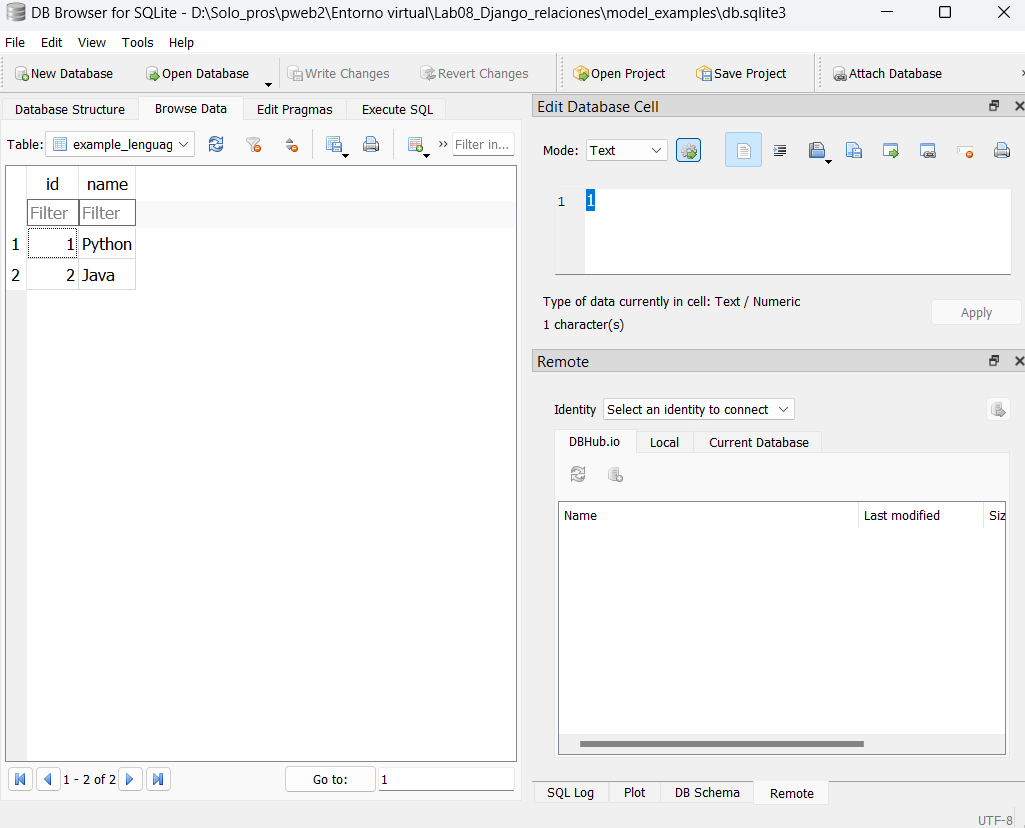
\includegraphics[width=1.0\textwidth,keepaspectratio]{img/C1.png}
		%\includesvg{img/automata.svg}
		%\label{img:mot2}
		%\caption{Product backlog.}
	\end{figure}
	\begin{figure}[H]
		\centering
		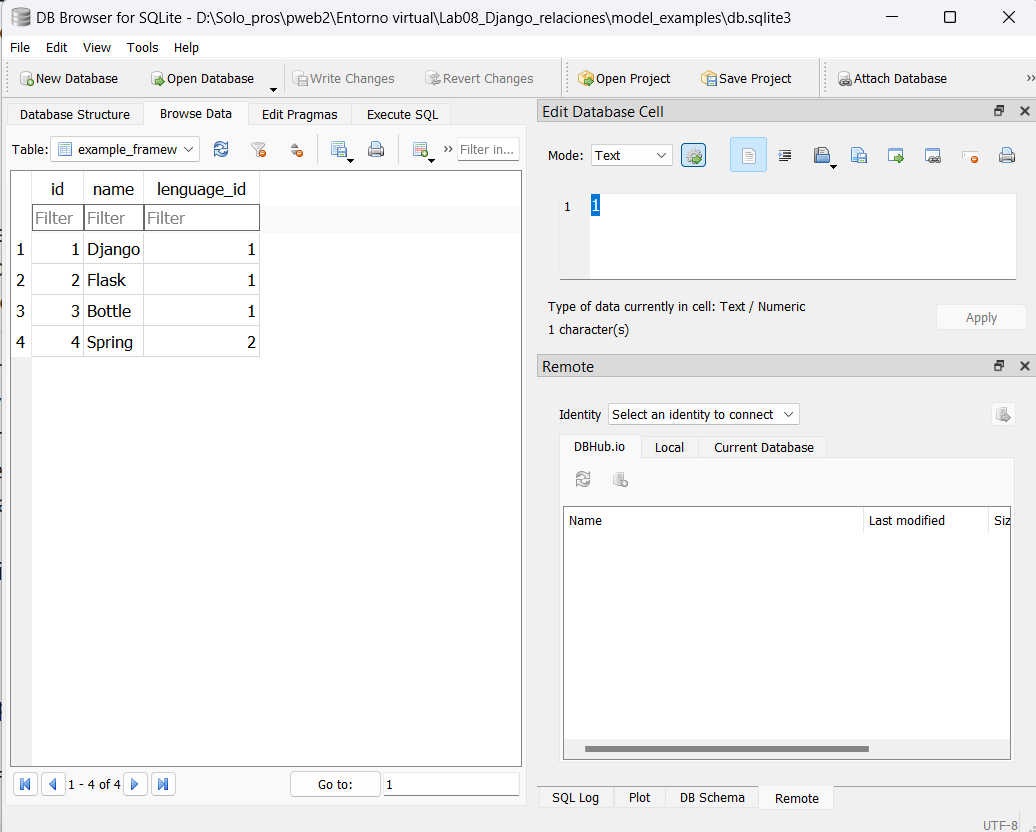
\includegraphics[width=1.0\textwidth,keepaspectratio]{img/C2.png}
		%\includesvg{img/automata.svg}
		%\label{img:mot2}
		%\caption{Product backlog.}
	\end{figure}
	\begin{figure}[H]
		\centering
		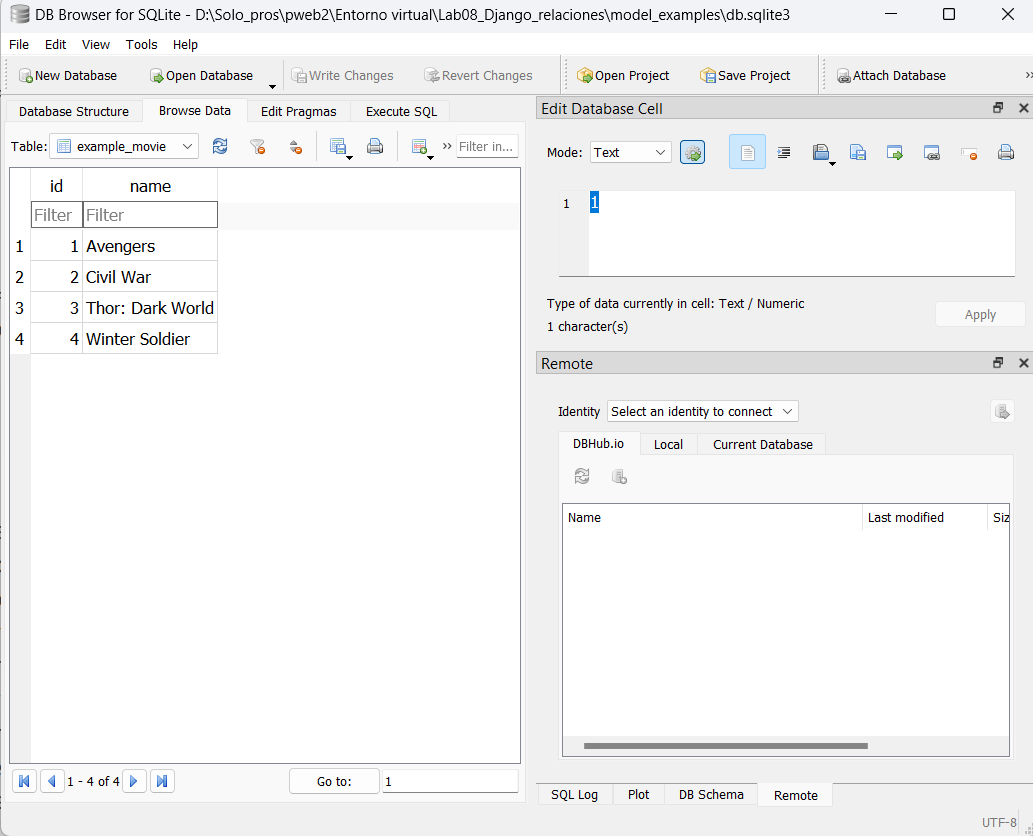
\includegraphics[width=1.0\textwidth,keepaspectratio]{img/C3.png}
		%\includesvg{img/automata.svg}
		%\label{img:mot2}
		%\caption{Product backlog.}
	\end{figure}
	\begin{figure}[H]
		\centering
		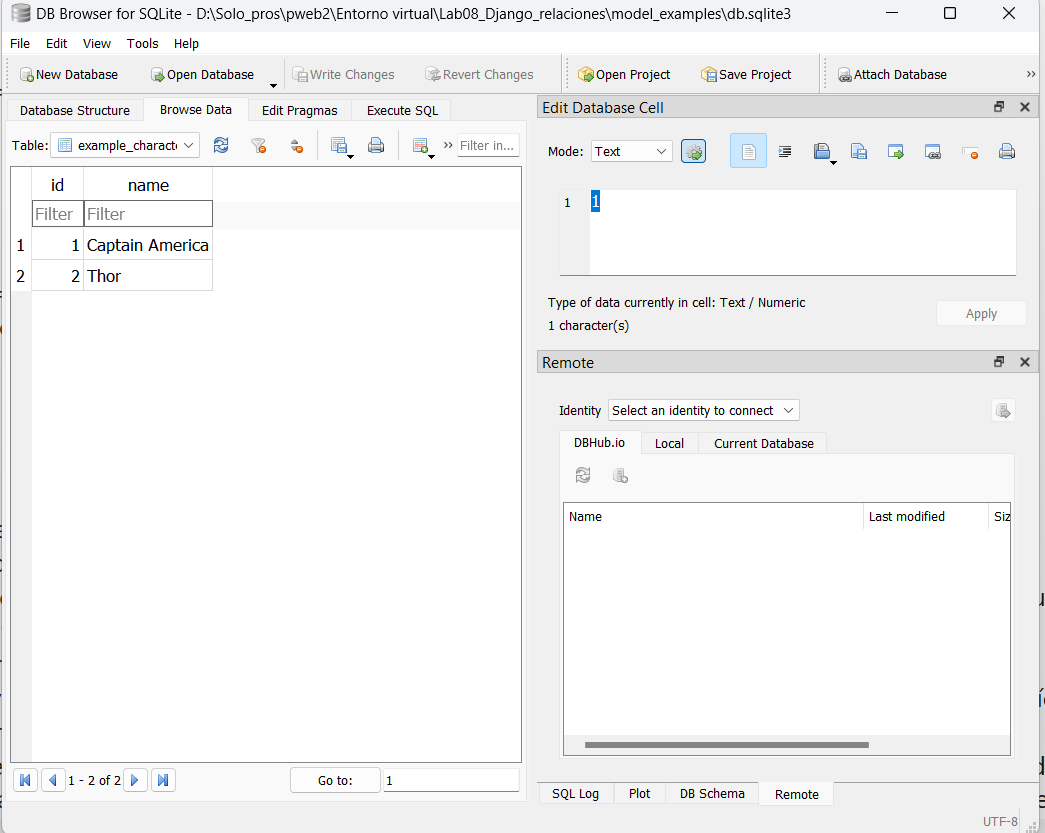
\includegraphics[width=1.0\textwidth,keepaspectratio]{img/C4.png}
		%\includesvg{img/automata.svg}
		%\label{img:mot2}
		%\caption{Product backlog.}
	\end{figure}
	\begin{figure}[H]
		\centering
		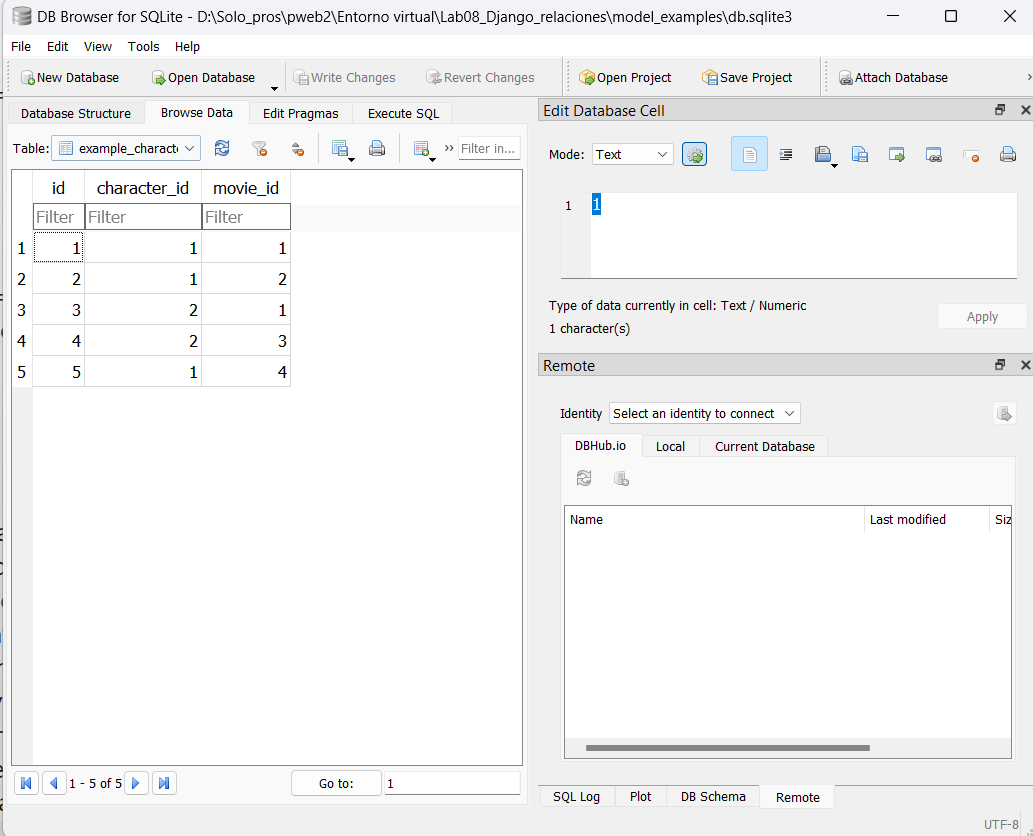
\includegraphics[width=1.0\textwidth,keepaspectratio]{img/C5.png}
		%\includesvg{img/automata.svg}
		%\label{img:mot2}
		%\caption{Product backlog.}
	\end{figure}	
\section{Impresion de pdf y envio de email en django}
	\begin{itemize}
		\item Instalamos xhtml12pdf para poder descargar pdfs
	\end{itemize}
	\begin{lstlisting}[language=bash,caption={Instalar xhtml12pdf}][H]
		pip install xhtml12pdf
	\end{lstlisting}
	\begin{itemize}
		\item Luego creamos views.py
	\end{itemize}	
	\lstinputlisting[language=Python, caption={Código de views.py},numbers=left,]{src/views.py}
	\begin{itemize}
		\item Generación de PDFs: Genera un PDF con datos de los modelos y descarga directamente (generar pdf) o envia por correo (enviar pdf por correo).
		\item Envío de correos: Enviar correos de texto plano o con un PDF adjunto, según lo que elija el usuario en el formulario (enviar correo).
		\item Los siguientes templates usados son:
	\end{itemize}	
	\lstinputlisting[language=html, caption={Código de views.py},numbers=left,]{src/enviar_correo.html}
	\lstinputlisting[language=html, caption={Código de views.py},numbers=left,]{src/plantilla_pdf.html}
	\begin{itemize}
		\item Se uso los datos creados en la base de datos para crear un pdf y enviarlo por correo
		\item Se ve de la siguiente manera:
	\end{itemize}	
	\begin{figure}[H]
		\centering
		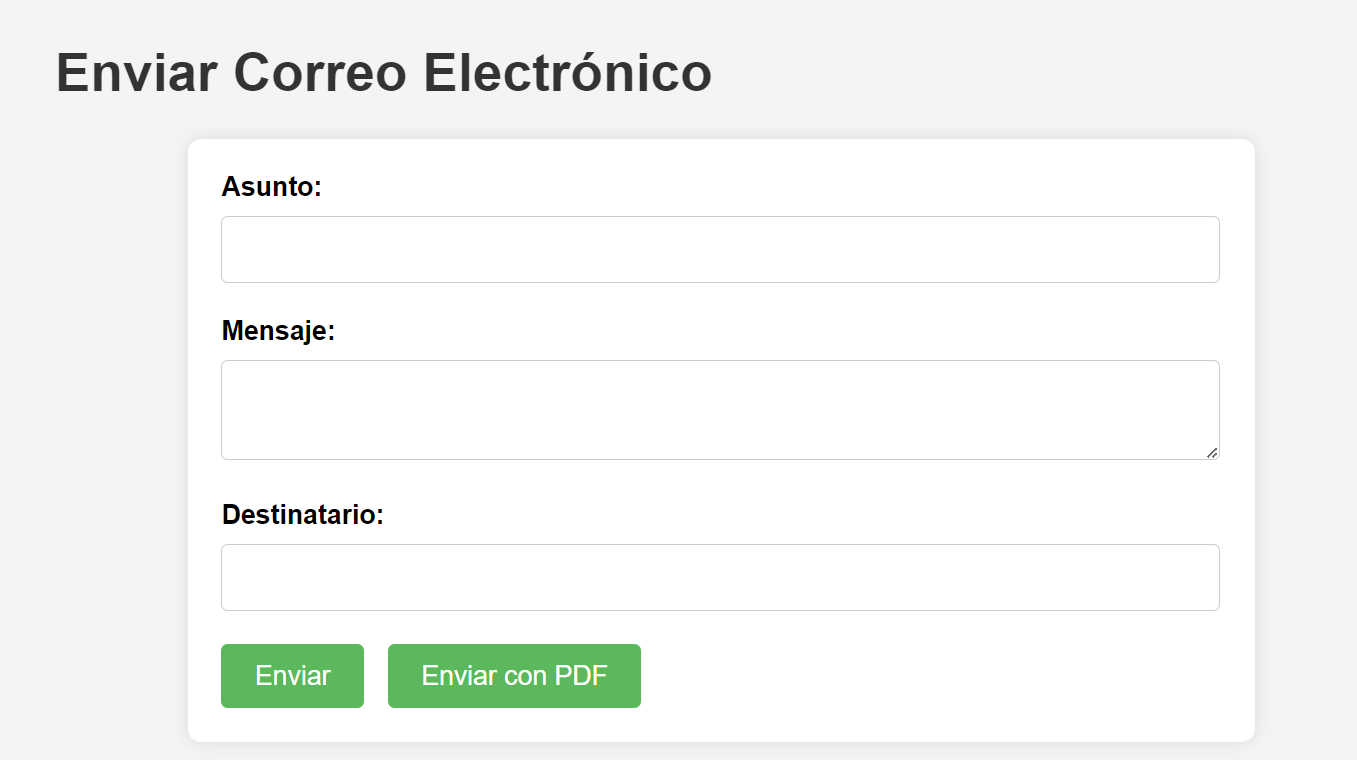
\includegraphics[width=1.0\textwidth,keepaspectratio]{img/C6.png}
		%\includesvg{img/automata.svg}
		%\label{img:mot2}
		%\caption{Product backlog.}
	\end{figure}
	\begin{figure}[H]
		\centering
		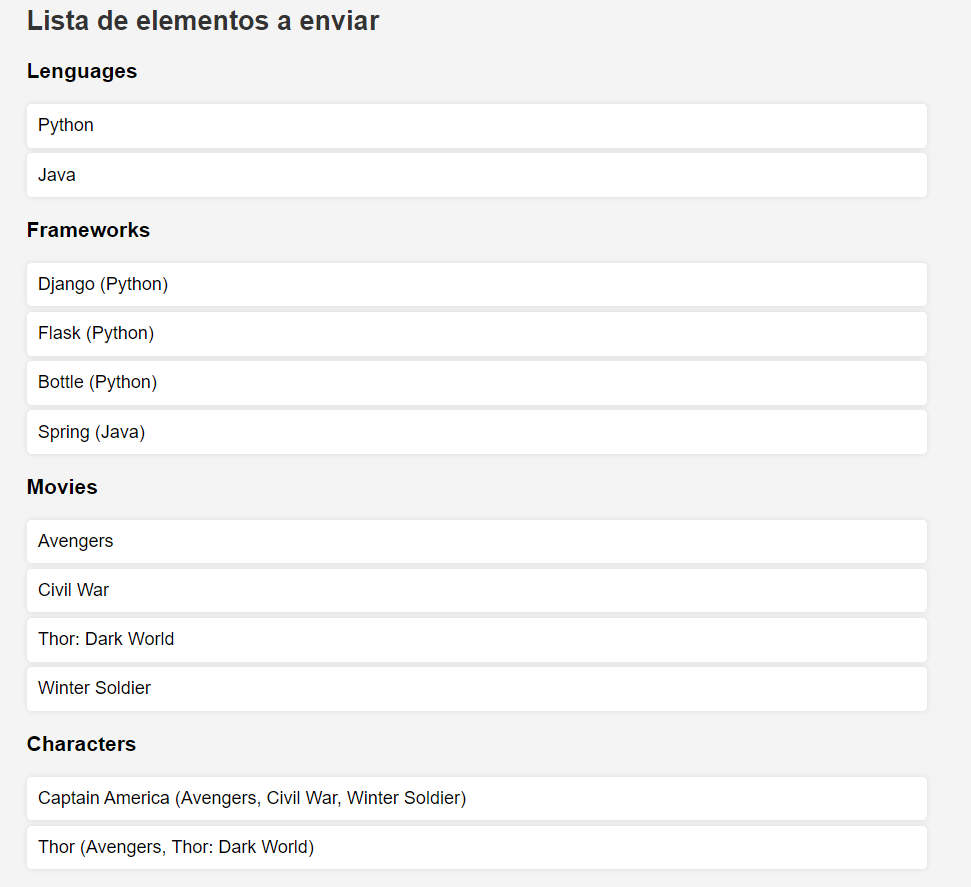
\includegraphics[width=1.0\textwidth,keepaspectratio]{img/C7.png}
		%\includesvg{img/automata.svg}
		%\label{img:mot2}
		%\caption{Product backlog.}
	\end{figure}	
\clearpage
\section{Referencias}
\begin{itemize}			
	\item \url{https://docs.djangoproject.com/es/3.2/}
	\item\url{https://docs.djangoproject.com/es/3.2/ref/models/fields/#field-types}
\end{itemize}	
	
%\clearpage
%\bibliographystyle{apalike}
%\bibliographystyle{IEEEtranN}
%\bibliography{bibliography}
			
\end{document}